\documentclass[11pt]{article}
\usepackage[margin=1.15in]{geometry}
\usepackage{amsmath,amssymb,graphicx,xcolor,booktabs,needspace,placeins,xurl}
\usepackage[hidelinks]{hyperref}
\newcommand{\E}{\mathbb{E}}
\emergencystretch=3em
\setlength{\parskip}{0.2em}
\renewcommand{\topfraction}{0.9}
\renewcommand{\bottomfraction}{0.8}
\renewcommand{\textfraction}{0.07}
\renewcommand{\floatpagefraction}{0.85}
\begin{document}
\begin{center}
{\LARGE Covariance comparisons using the complete measured samples\par}
\vspace{0.6em}
{\large Direct simulations, second-order Eifler correction,\par}
{\large and the released DES Y3 covariance\par}
\vspace{0.5em}
21 November 2026
\end{center}

\section{Two comparisons and the data used in each}
\paragraph{The first comparison uses all available measured aperture vectors.}
We estimate a covariance directly from all 15,997 measured simulation files.
We then use that same sample covariance in the second-order
Friedrich--Eifler precision expansion~\cite{pme}, keeping its starting matrix
fixed. After checking that the corrected precision is positive definite,
we invert it to obtain a covariance for comparison. Both calculations use
the same sixteen measured quantities and the same complete sample.
There is no calibration/correction/validation partition in this experiment.

\paragraph{The second comparison uses matched rows of the released DES covariance.}
Our existing pair-counting calculation measures four published $\xi_+$
angular bins from 32 primary run labels. We use all 32 vectors to estimate
their covariance and compare it with the corresponding released DES
submatrix. This four-bin measurement has not been performed on all 15,997
maps. It is also a different statistic from the sixteen aperture moments.
The two comparisons answer different questions and their matrices must not
be compared entry by entry.

\paragraph{What the comparisons show.}
For the complete aperture sample, the Eifler covariance has per-row standard
deviations about 11--13\% larger for the squared moments, while changes for
the cubed moments range from about $-0.1\%$ to $+1.4\%$. Correlation
coefficients differ by as much as 0.199. The difference persists largely
because a second-order inverse expansion is truncated. For the separate
four-bin DES comparison, the measured variances range from about 1.05 to
1.81 times the released values, with appreciable uncertainty from the
32-map sample. Neither comparison alone identifies the unknown true
covariance or validates cosmological parameter errors.

\paragraph{Reproduction and credits.}
The \href{EXAMPLE_COVARIANCE_COMPARISON.ipynb}{companion notebook} beside
this note computes both comparisons and the difference and split-triangle
plots. Small recorded matrices and vectors reproduce its outputs without
loading the simulation archive. Its optional controls recompute the full
sample covariance from the saved measurement table and repeat the bounded
pair measurements. \textbf{We thank Rafael Gomes for the maps and analysis
products, Oliver Friedrich and Tim Eifler for the precision expansion,
and Mike Jarvis and the TreeCorr contributors for the pair-counting code.}
The DES science context and released analysis are described by
Gomes et al.~\cite{gomes}.

\section{Define the complete-sample aperture covariance}
\paragraph{A map supplies values on the retained DES footprint.}
Each file has four source-bin slots, two shear-component slots and 369,190
retained pixel positions. The companion \nolinkurl{indices_512.npy} gives
the HEALPix pixel IDs. The maps are NSIDE 512; RING ordering and equatorial
coordinates are inferred from the footprint geometry. The shear basis and
source-bin order still require their producer record. The calculation uses
one fixed pixel interpretation for every method.

\paragraph{The sixteen rows are coarse moments, with an explicit ordering.}
A tangential-shear filter with radius 30 or 60 arcminutes is integrated
around 64 fixed centers in each source-bin slot. Let $a_{bRc}$ be the
resulting aperture value for source bin $b$, radius $R$ and center $c$.
For each source bin and radius, the squared-moment row is
\begin{equation}
 d_{2,bR}=\frac{1}{64}\sum_{c=1}^{64}a_{bRc}^2.
\end{equation}
The separate cubed-moment row is
\begin{equation}
 d_{3,bR}=\frac{1}{64}\sum_{c=1}^{64}a_{bRc}^3.
\end{equation}
The first eight rows contain the squared moments: source 1 at the two
radii, then source 2, and so on. The next eight rows contain the cubed
moments in the same source/radius order. The complete covariance retains
the correlations within and between these blocks. These raw moments keep
noise self-products and use equal pixel weights. They are a diagnostic of
the maps, not the published finite-triangle Map3 estimator or the published
xi/Map3 data vector.

\paragraph{Every available file enters the direct covariance.}
The settled local inventory has 15,997 maps, with run labels 0--199,
four cut labels and twenty realization labels. Three combinations of those
observed labels are absent: run 168/cut 2/draws 7 and 19, and
run 168/cut 3/draw 19. All present files were measured. Their small
sixteen-row vectors are stored separately from the maps; the full generated
measurement tables occupy about 12 MB. File labels do not by themselves
establish independent skies or producer-certified completeness.

\paragraph{Compute a covariance of one measurement, not of its average.}
Let $d_s$ be the sixteen-component vector from file $s$ and let
$N=15997$. First form its mean over files:
\begin{equation}
 \bar d=\frac{1}{N}\sum_{s=1}^{N}d_s.
\end{equation}
Subtract that mean to obtain one residual vector per file:
\begin{equation}
 e_s=d_s-\bar d.
\end{equation}
The outer product of a residual with itself records which rows fluctuate
together. Averaging these outer products gives
\begin{equation}
 C_{\rm sim}=\frac{1}{N-1}\sum_{s=1}^{N}e_s e_s^{\mathsf T}.
 \label{eq:sample}
\end{equation}
This is the direct empirical covariance used throughout the first
comparison. It is not divided again by $N$. Such a division would change
the quantity into a covariance of the mean under independence, rather
than the fluctuations of a single measured vector.

\section{Use the same sample in the Eifler calculation}
\paragraph{Keep the starting matrix fixed.}
Denote the existing Gaussian moment reference by $M$. It is the previously
recorded starting matrix; there is no new reference fit or allocation of
simulations to a calibration group. Its entries were constructed from
Gaussian pair contractions of aperture covariances, so it is not a
noise-free, survey-matched analytic CosmoLike covariance. The present
question is what the correction does to this fixed matrix when supplied
with the entire measured sample.

\paragraph{First express the sample covariance in reference units.}
Factor the positive reference matrix into
\begin{equation}
 M=L L^{\mathsf T}.
\end{equation}
For one scalar observable, dividing a residual by its reference standard
deviation makes it dimensionless. The matrix version also accounts for
correlations. Its covariance is
\begin{equation}
 S=L^{-1}C_{\rm sim}L^{-\mathsf T}.
\end{equation}
If the sample covariance exactly equaled the reference, $S$ would be the
identity. Departures from the identity are what the expansion corrects.

\paragraph{Correct the noisy matrix square before using the second-order term.}
For independent Gaussian summary vectors, the sample-covariance moments
obey the Wishart identities used by Friedrich and Eifler. The corrected
square is
\begin{equation}
 Q=\frac{\nu^2 S^2-\nu S\operatorname{tr}(S)}{\nu^2+\nu-2}.
 \label{eq:quadratic}
\end{equation}
Here $S^2$ means matrix multiplication, not squaring each entry.
The trace is the sum of the diagonal entries. The subtraction removes the
mean noise contribution that otherwise remains when a noisy matrix is
multiplied by itself, provided the stated sampling assumptions apply.
The notebook calculates the square, trace term and normalization explicitly
before checking the shared statistical routine.

\paragraph{State the count convention without assigning independence to filenames.}
For this requested complete-file comparison, Equation~\eqref{eq:quadratic}
is evaluated with nominal
\begin{equation}
 \nu=N-1=15996.
\end{equation}
Related maps are not established to be independent, and these nonlinear
summary moments are not established to be Gaussian. This count therefore
defines a formal all-file evaluation of the formula; it is not a validated
independent-simulation degree of freedom. The unbiasedness guarantee does
not follow for the archive merely because the matrix arithmetic can be
performed. No effective independent count is inferred or fitted here.

\paragraph{Construct a precision and then return to covariance units.}
The second-order polynomial in reference coordinates is
\begin{equation}
 P_2=3I-3S+Q.
\end{equation}
Its smallest eigenvalue in this calculation is about 0.8204, so it is
positive definite. Restoring the original units gives the precision
\begin{equation}
 \Psi_{\rm E}=L^{-\mathsf T}P_2L^{-1}.
\end{equation}
A precision is an inverse covariance. We therefore compare the direct
simulation covariance with
\begin{equation}
 C_{\rm E}=\Psi_{\rm E}^{-1}.
\end{equation}
Both displayed matrices are positive definite. No eigenvalue is clipped,
no scalar rescaling is fitted, and no data row is removed to obtain this
property.

\section{Read the complete-sample covariance plots}
\paragraph{A stable difference normalization.}
The matrix difference in Figure~\ref{fig:all-difference} is normalized by
the direct simulation standard deviations:
\begin{equation}
 \Delta_{ij}=100\,
 \frac{(C_{\rm E}-C_{\rm sim})_{ij}}
 {\sqrt{(C_{\rm sim})_{ii}(C_{\rm sim})_{jj}}}.
\end{equation}
On the diagonal this is the percentage change in variance. Off the diagonal
it remains finite when a reference covariance entry is close to zero.
Dividing instead by each individual off-diagonal entry would exaggerate
small differences near correlation zero crossings. The histogram describes
all 256 entries, including symmetric duplicates; its bars are not independent
statistical measurements.

\begin{figure}[htbp]
 \centering
 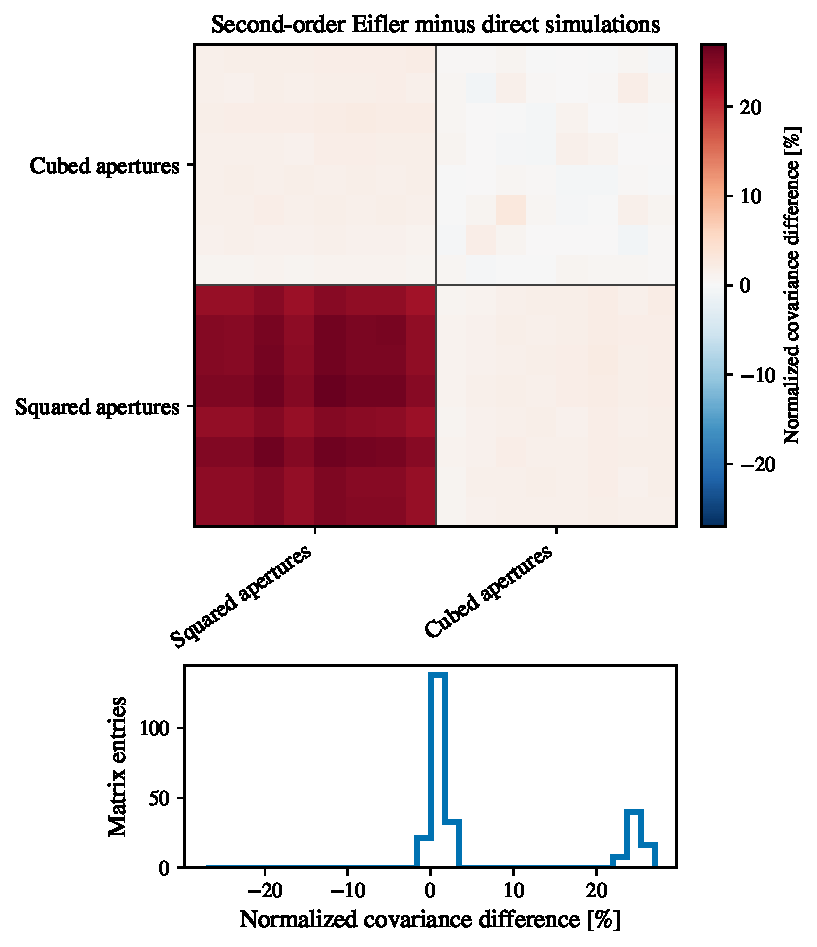
\includegraphics[width=0.76\linewidth]{plots/all_difference/all_difference.pdf}
 \caption{Eifler minus direct simulation covariance, using the same 15,997
 vectors. The normalization uses the direct simulation diagonal. The lower
 panel shows the distribution of matrix entries, including symmetric copies.}
 \label{fig:all-difference}
\end{figure}

\paragraph{Separate variance changes from correlation changes.}
For each method, a correlation coefficient divides its covariance entry
by its own two standard deviations:
\begin{equation}
 R_{ij}=\frac{C_{ij}}{\sqrt{C_{ii}C_{jj}}}.
\end{equation}
Figure~\ref{fig:all-triangles} puts the Eifler correlation in the displayed
upper-left triangle and the direct simulation correlation in the lower-right.
Thus every symmetric pair compares two methods at the same row labels.
Each half uses its own diagonal normalization; the diagonal is one for both.
The plotting convention places increasing row index upward, which is why
we name the displayed halves explicitly.

\begin{figure}[htbp]
 \centering
 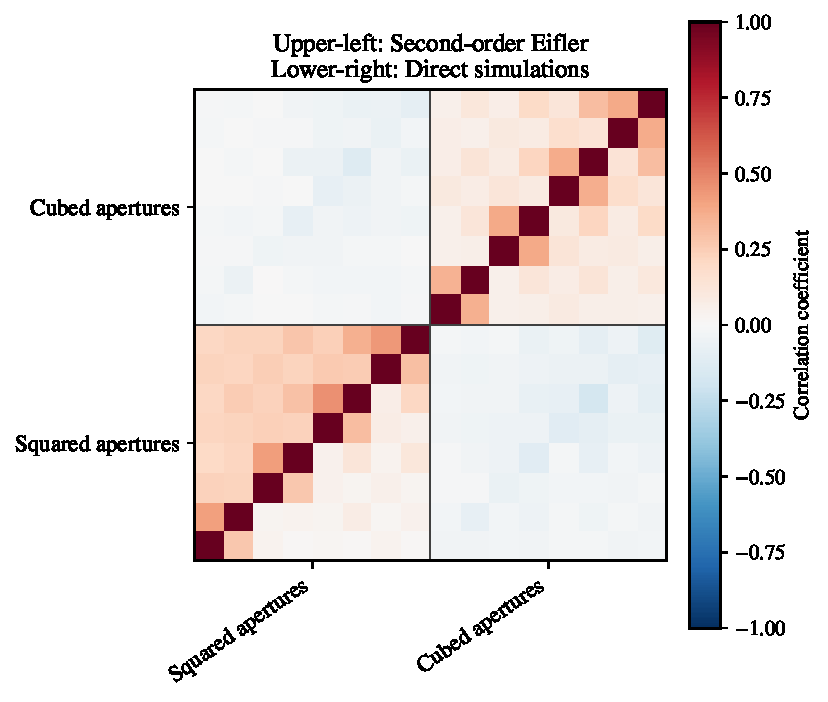
\includegraphics[width=0.88\linewidth]{plots/all_triangles/all_triangles.pdf}
 \caption{Correlation coefficients for the complete aperture sample.
 Upper-left: second-order Eifler. Lower-right: direct simulation covariance.
 The block boundary separates the eight squared and eight cubed moments.}
 \label{fig:all-triangles}
\end{figure}

\FloatBarrier
\paragraph{The numerical size of the difference.}
Per-row standard deviations, obtained by taking square roots of covariance
diagonal entries, increase by 10.8--12.5\% for the squared moments.
For the cubed moments the changes range from $-0.12\%$ to $+1.44\%$.
The normalized covariance differences range from about $-0.78\%$ to
$+26.64\%$, and the largest absolute correlation-coefficient change is
0.199. Variance percentages and standard-deviation percentages differ
because one is the square of the other.

\paragraph{A sample used by both methods is not an independent validation set.}
Multiplying $C_{\rm sim}$ by its own exact inverse necessarily gives the
identity. The corresponding trace per row is one by algebra, not evidence
that the covariance is cosmologically accurate. The Eifler precision times
that same covariance has trace per row about 0.9583. This describes an
average difference in weighting between the estimators. It is not a held-out
accuracy score, and different matrix directions can cancel in its average.

\FloatBarrier
\section{Why the difference remains with many measured files}
\paragraph{An infinite convergent series need not be accurate at second order.}
To isolate truncation, temporarily omit the finite-$N$ square subtraction
and use $Q=S^2$. Along a direction where $S$ has eigenvalue $\lambda$, the
second-order precision polynomial becomes
\begin{equation}
 p_2(\lambda)=3-3\lambda+\lambda^2.
\end{equation}
The exact inverse of that sample direction is $1/\lambda$. Hence the
second-order weight relative to the direct inverse is
\begin{equation}
 \lambda p_2(\lambda)=1+(\lambda-1)^3.
\end{equation}
The smallest measured eigenvalue is approximately 0.168. Substitution gives
a relative weight near 0.424. Inverting that weight gives a covariance
ratio near 2.36 along that particular combination of rows. Individual
diagonal entries mix many directions, so their changes can be smaller.

\paragraph{Distinguish that truncation from the finite-sample square term.}
The largest absolute departure of an eigenvalue of $S$ from one is
about 0.832. This number is the residual spectral radius. Being below
one, it indicates convergence of the infinite inverse series for the sample
matrix, but does not make the second-order term exact. With the nominal
count used here, including Equation~\eqref{eq:quadratic} changes standard
deviations by only 0.029--0.061\% relative to the uncorrected second-order
polynomial. Most of the displayed difference is therefore finite-order
truncation at the current $S$ and $M$. Increasing the sample size does not,
by itself, remove an algebraic truncation at fixed matrices.

\paragraph{Does fourth order solve the truncation?}
A check with these same matrices, omitting finite-sample corrections at
both orders, gives a partial improvement. Define the residual matrix
\begin{equation}
 U=I-S.
\end{equation}
Keeping two additional terms gives the fourth-order polynomial
\begin{equation}
 P_4=I+U+U^2+U^3+U^4.
\end{equation}
Its squared-moment standard deviations differ from the direct covariance
by 5.4--6.3\%, compared with 10.7--12.5\% at second order in this
uncorrected-polynomial check. The weakest direction still receives only
about 0.601 times its exact sample-inverse weight: a discrepancy of about
40\%. Fourth order helps, but improving the starting covariance remains
necessary for a reliable low-order approximation. This calculation isolates
truncation; it is not an unbiased fourth-order estimator. Noisy cubic and
quartic powers require their own noise-bias corrections. The companion
notebook reproduces this check without changing the displayed second-order
comparison or partitioning the sample.

\section{Compare with the released DES covariance}
\paragraph{Use matching observed-row definitions.}
The released joint matrix has 480 rows: 200 for $\xi_+$, 200 for $\xi_-$
and 80 for Map3. We select source-bin slot four paired with itself and
joint rows 192--195, counted from zero. Their four angular bins span
39.622--99.527 arcminutes. TreeCorr~\cite{treecorr} measures those same
bins in runs 0--31, cut zero and realization zero. All 32 resulting vectors
enter their sample covariance through Equation~\eqref{eq:sample}, with
$N=32$ and four rows instead of sixteen. There is no split of those runs.

\paragraph{Control the pair calculation before interpreting the matrices.}
Angular-bin and shear-angle approximation tolerances are both zero.
A 2,048-pixel subset agrees with direct pair enumeration for both tested
shear-sign choices. Cross-correlating two catalogue copies of one field
also recovers its auto-correlation, and a different-field cross check agrees
with direct pairs. We use the explicit provisional east/north shear
convention, converted to TreeCorr's west/north basis with
\nolinkurl{flip_g2=True}. The notebook retains the alternative-sign check.
Equal pixel weights, the source-bin and shear conventions, and the
NSIDE 512 versus the methods paper's NSIDE 1024 remain physical matching
questions. Numerical agreement of pair algorithms cannot resolve them.

\paragraph{Show the same two matrix comparisons.}
Figure~\ref{fig:des-difference} uses the released diagonal to normalize
measured-minus-released differences. Figure~\ref{fig:des-triangles} shows
one correlation triangle from each method. These figures use four
$\xi_+$ rows only. The sixteen-row aperture covariance above is never
substituted for those rows or matched to the 480-row release by its dimensions.

\begin{figure}[htbp]
 \centering
 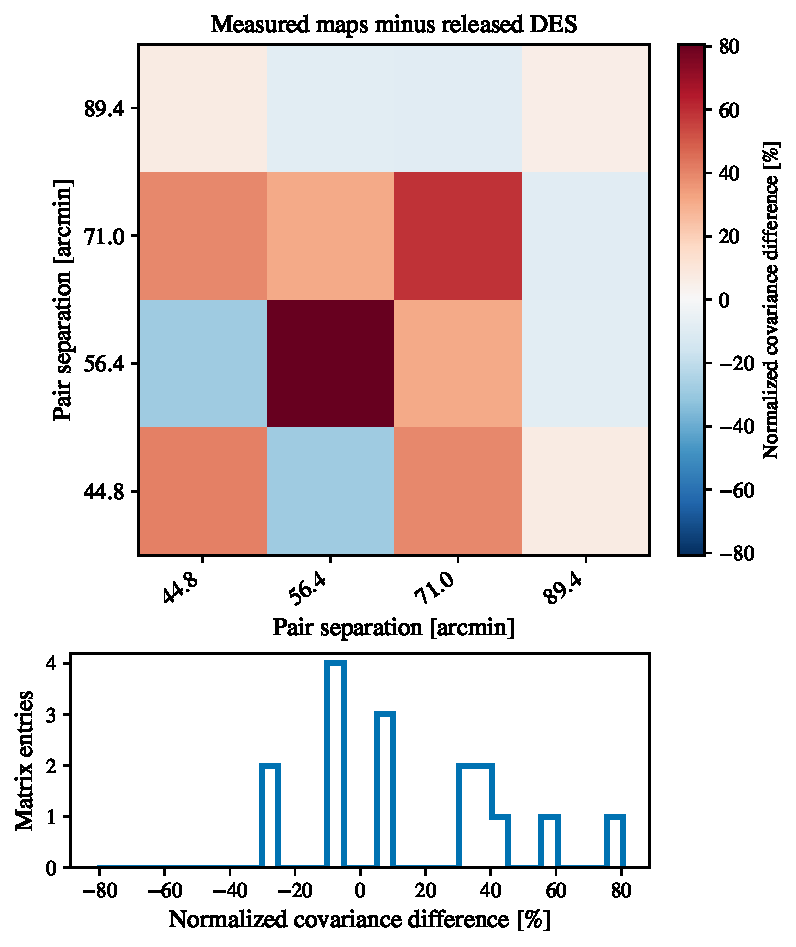
\includegraphics[width=0.76\linewidth]{plots/des_difference/des_difference.pdf}
 \caption{Measured minus released covariance for four matching $\xi_+$ bins.
 The denominator uses the released DES diagonal. The measured matrix uses
 all 32 available pair-measurement vectors; its sampling noise remains.}
 \label{fig:des-difference}
\end{figure}

\begin{figure}[htbp]
 \centering
 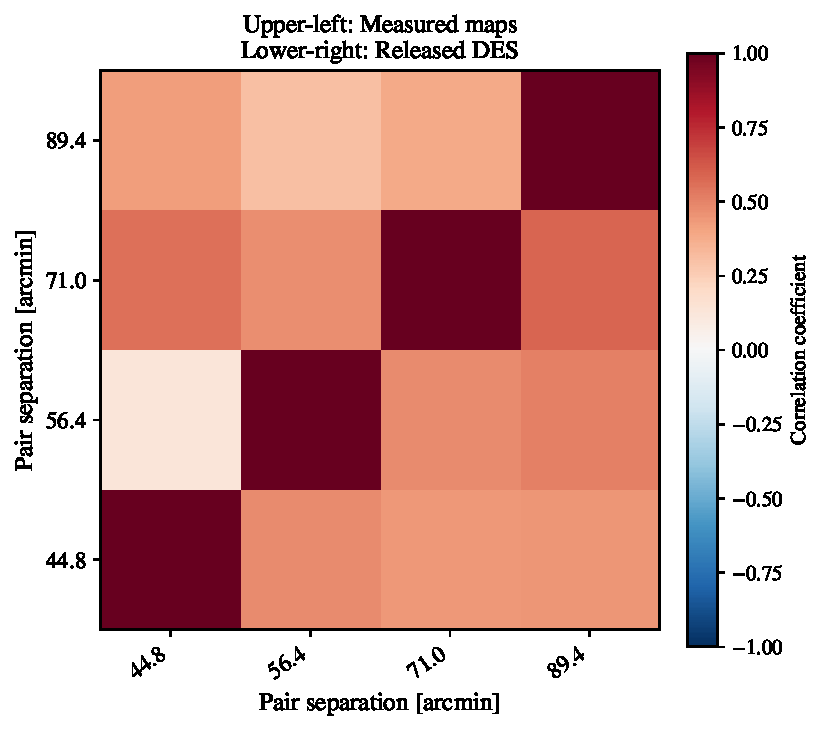
\includegraphics[width=0.88\linewidth]{plots/des_triangles/des_triangles.pdf}
 \caption{Four-bin correlation comparison. Upper-left: measured maps.
 Lower-right: released DES joint covariance. Axis labels give the published
 mean pair separations in arcminutes.}
 \label{fig:des-triangles}
\end{figure}

\FloatBarrier
\paragraph{Keep the sampling uncertainty visible.}
The four variance ratios are approximately 1.41, 1.81, 1.58 and 1.05.
To estimate their sensitivity to the 32-run sample, remove one run, recompute
the ratio and repeat for each run. If $r_i^{(-s)}$ is the result after omitting
run $s$, average those leave-one-out values:
\begin{equation}
 \bar r_i^{\rm jack}=\frac{1}{N}\sum_s r_i^{(-s)}.
\end{equation}
Their jackknife variance is
\begin{equation}
 \widehat{\mathrm{Var}}_{\rm jack}(r_i)
 =\frac{N-1}{N}\sum_s(r_i^{(-s)}-\bar r_i^{\rm jack})^2.
\end{equation}
The resulting standard errors are about 0.37, 0.42, 0.45 and 0.28,
shown in Figure~\ref{fig:variance}. These condition on independent run
labels and a fixed released reference. They do not include uncertainty in
that reference or estimator mismatch. Angular bins are correlated; the
four differences cannot be treated as four independent significance tests.

\begin{figure}[htbp]
 \centering
 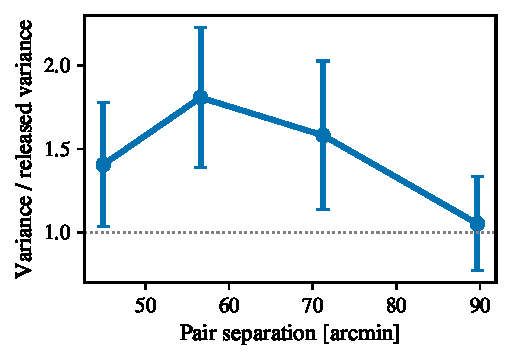
\includegraphics[width=0.72\linewidth]{plots/variance/variance.pdf}
 \caption{Single-survey variance relative to the released joint covariance.
 The dotted line marks equality. Error bars are leave-one-run-out standard
 errors, with the released matrix held fixed.}
 \label{fig:variance}
\end{figure}

\FloatBarrier
\paragraph{The correlations add information beyond the diagonal ratios.}
The largest absolute correlation difference is about 0.355. Expressing the
measured covariance in units of the released covariance gives eigenvalues
approximately 0.80, 1.05, 2.18 and 2.87. Equality would give four ones.
The ordered eigenvalue extremes are noisy with 32 samples. They identify
what needs a better matched comparison; they do not by themselves assign
a statistical significance to a physical discrepancy.

\FloatBarrier
\section{Input provenance and reproduction}
\paragraph{The released files are related, but are not interchangeable.}
The last 80-by-80 block of the joint covariance equals the standalone Map3
covariance exactly. The standalone two-point covariance differs from the
joint matrix's first 400-by-400 block: their diagonal ratios range from
0.895 to 1.092. We consistently use the joint matrix. Its FITS header says
\nolinkurl{NSIM=500}, whereas the selected paired likelihood configuration
uses 796 covariance realizations. The notebook reads and prints both
values from the actual files. Their production history is needed to resolve
that discrepancy; neither input has been changed.

\paragraph{What remains to be supplied by the map producer.}
The definitions of \nolinkurl{run}, \nolinkurl{ncut} and \nolinkurl{nreal}
are needed to interpret file dependence and noise. We also need the shear
basis, source-bin order, catalogue weights and pixel occupancies, and the
relationship between these NSIDE 512 maps and the maps used for the released
covariance. The local run labels extend from 0 to 199, while the methods
paper describes 199 parent full skies and four footprints per sky. A label
count alone does not establish that mapping. These questions concern how
to interpret the matrices, not whether the comparisons can be reproduced.

\paragraph{Where the calculations live.}
The companion \nolinkurl{EXAMPLE_COVARIANCE_COMPARISON.ipynb} is beside
this note. Its compact inputs are under
\nolinkurl{tests/covariance_map_comparison/}. The file
\nolinkurl{all_maps_covariance.txt} stores the direct sixteen-row covariance,
and \nolinkurl{aperture_reference.txt} stores the fixed starting matrix.
The full per-file measurement table remains under
\nolinkurl{chains/covariance_maps_full/}; the notebook can verify the
recorded covariance against it without reopening the maps.
The four-bin records are in the same small test-data folder, and
\nolinkurl{data/y3_observed_manifest.yaml} records the pinned released
FITS inputs. Figure folders beside the note contain text matrices and
standalone redrawing scripts. No raw simulation array is committed.

\begin{thebibliography}{9}
\bibitem{pme} O. Friedrich and T. Eifler,
\emph{Precision matrix expansion --- efficient use of numerical simulations
in estimating errors on cosmological parameters},
\href{https://arxiv.org/abs/1703.07786}{arXiv:1703.07786}.
\bibitem{gomes} R. C. H. Gomes et al.,
\emph{Cosmology with second and third-order shear statistics for the Dark
Energy Survey: Methods and simulated analysis},
\href{https://arxiv.org/abs/2503.03964}{arXiv:2503.03964}, version 2.
Inputs: \href{https://github.com/rchgomes/3pcf_integrator}
{rchgomes/3pcf\_integrator}.
\bibitem{treecorr} M. Jarvis and contributors,
\href{https://rmjarvis.github.io/TreeCorr/_build/html/shear.html}
{TreeCorr shear conventions} and
\href{https://rmjarvis.github.io/TreeCorr/_build/html/gg.html}
{GGCorrelation documentation}.
\end{thebibliography}
\end{document}
